%% DONE
\newpage
\let\cleardoublepage\clearpage
\chapter{Горное и нефтегазовое дело}
\ID{МРНТИ 52.01.93}{}

\begin{articleheader}
\sectionwithauthors{A.R. Ensebayeva, A.M. Kurmanov, D. Kazbekova, Sh. Aitimova, L. Yedilbayeva}{TRANSFORMATION OF LABOR PROTECTION MECHANISMS IN HAZARDOUS PRODUCTION CONDITIONS: KAZAKHSTAN' S TRANSITION TO MODERN RISK-BASED APPROACHES}

{\bfseries
\textsuperscript{1}A.R. Ensebayeva\textsuperscript{\envelope }\authorid
\textsuperscript{1}A.M. Kurmanov\authorid,
\textsuperscript{2} D. Kazbekova\authorid,
\textsuperscript{1}Sh. Aitimova\authorid,
\textsuperscript{3}L. Yedilbayeva\authorid}
\end{articleheader}

\begin{affiliation}
\emph{\textsuperscript{1}Republican Research Institute for labor protection of the Ministry of Labor and social protection of the population of the Republic of Kazakhstan, Astana, Kazakhstan,}

\emph{\textsuperscript{2}Institute of Industrial Ecological Sciences (IIES) of the University of Occupational and Environmental Health, Japan,}

\emph{\textsuperscript{3}Republican Research Institute for labor protection of the Ministry of Labor and social protection of the population of the Republic of Kazakhstan, Almaty, Kazakhstan}

\raggedright \textsuperscript{\envelope }{\em Correspondent-author: \href{mailto:nel1212kz@gmail.com}{\nolinkurl{nel1212kz@gmail.com}}}
\end{affiliation}

The article is devoted to the analysis of problems and opportunities of
increasing social guarantees for workers of hazardous industries in
Kazakhstan. Particular attention is paid to the lack of a unified
approach to workplace certification and assessment of working
conditions, which leads to inconsistency and bias in assessing
occupational risks. The current system is criticized for the lack of
standardized criteria and insufficient control. The article offers
recommendations on the development of new legislative acts for the
standardization of workplace certification, professional development of
occupational safety specialists and the creation of effective feedback
mechanisms for employees. The introduction of a differentiated approach
to social guarantees depending on industry risks and compliance of
Kazakhstani standards with international requirements are also being
considered. The economic aspects of the proposed changes and the need
for cooperation between government, industry and workers to effectively
implement safety measures and improve working conditions are discussed.

{\bfseries Keywords:} social guarantees, harmful and dangerous working
conditions, compensation, labor protection, certification of workplaces,
working conditions.

\begin{articleheader}
{\bfseries ТРАНСФОРМАЦИЯ МЕХАНИЗМОВ ОХРАНЫ ТРУДА В ОПАСНЫХ ПРОИЗВОДСТВЕННЫХ УСЛОВИЯХ: ПЕРЕХОД КАЗАХСТАНА К СОВРЕМЕННЫМ РИСК-ОРИЕНТИРОВАННЫМ ПОДХОДАМ}

{\bfseries
\textsuperscript{1}А.Р. Енсебаева\textsuperscript{\envelope },
\textsuperscript{1}А. М. Курманов,
\textsuperscript{2}Д.Б. Казбекова,
\textsuperscript{1}Ш.Т. Айтимова,
\textsuperscript{3}Л. Едильбаева}
\end{articleheader}

\begin{affiliation}
\emph{\textsuperscript{1}Республиканский научно-исследовательский институт по охране труда Министерства труда и социальной защиты населения Республики Казахстан, Астана, Казахстан,}

\emph{\textsuperscript{2}Институт промышленных экологических наук (IIES) Университета гигиены труда и окружающей среды, Япония,}

\emph{\textsuperscript{3}Республиканский научно-исследовательский институт по охране труда Министерства труда и социальной защиты населения Республики Казахстан, Алматы, Казахстан,}

\emph{e-mail: \href{mailto:nel1212kz@gmail.com}{\nolinkurl{nel1212kz@gmail.com}}}
\end{affiliation}

Статья посвящена анализу проблем и возможностей повышения социальных
гарантий работников опасных производств в Казахстане. Особое внимание
уделено отсутствию единого подхода к сертификации рабочих мест и оценке
условий труда, что приводит к непоследовательности и необъективности в
оценке профессиональных рисков. Критикуется действующая система за
отсутствие стандартизированных критериев и недостаточный контроль. В
статье предлагаются рекомендации по разработке новых законодательных
актов для стандартизации сертификации рабочих мест, повышению
квалификации специалистов по охране труда и созданию эффективных
механизмов обратной связи для работников. Также рассматривается
внедрение дифференцированного подхода к социальным гарантиям в
зависимости от отраслевых рисков и соответствие казахстанских стандартов
международным требованиям. Обсуждаются экономические аспекты
предложенных изменений и необходимость сотрудничества между
правительством, промышленностью и работниками для эффективного внедрения
мер безопасности и улучшения условий труда.

{\bfseries Ключевые слова:} социальные гарантии, вредные и опасные условия
труда, компенсации, охрана труда, аттестация рабочих мест, условия труда

\begin{articleheader}
{\bfseries ҚАУІПТІ ӨНДІРІСТІК ЖАҒДАЙЛАРДА ЕҢБЕКТІ ҚОРҒАУ ТЕТІКТЕРІН ТРАНСФОРМАЦИЯЛАУ: ҚАЗАҚСТАННЫҢ ҚАЗІРГІ ЗАМАНҒЫ ТӘУЕКЕЛГЕ БАҒДАРЛАНҒАН ТӘСІЛДЕРГЕ КӨШУІ}

{\bfseries
\textsuperscript{1}А.Р. Енсебаева\textsuperscript{\envelope },
\textsuperscript{1}А. М. Курманов,
\textsuperscript{2}Д.Б. Казбекова,
\textsuperscript{1}Ш.Т. Айтимова,
\textsuperscript{3}Л. Едильбаева}
\end{articleheader}

\begin{affiliation}
\emph{\textsuperscript{1}Қазақстан Республикасы Еңбек және халықты әлеуметтік қорғау министрлігінің Еңбекті қорғау жөніндегі республикалық ғылыми-зерттеу институты, Астана, Қазақстан,}

\emph{\textsuperscript{2}Өндірістік экологиялық ғылымдар институты (iies) Еңбек және қоршаған ортаны қорғау Университеті, Жапония,}

\emph{\textsuperscript{3}Қазақстан Республикасы Еңбек және халықты әлеуметтік қорғау министрлігінің Еңбекті қорғау жөніндегі республикалық ғылыми-зерттеу институты, Алматы, Қазақстан,}

\emph{e-mail: \href{mailto:nel1212kz@gmail.com}{\nolinkurl{nel1212kz@gmail.com}}}
\end{affiliation}

Мақала Қазақстандағы қауіпті өндіріс қызметкерлерінің әлеуметтік
кепілдіктерін арттыру мәселелері мен мүмкіндіктерін талдауға арналған.
Жұмыс орындарын сертификаттауға және еңбек жағдайларын бағалауға
бірыңғай көзқарастың болмауына ерекше назар аударылады, бұл кәсіби
тәуекелдерді бағалауда сәйкессіздік пен біржақтылыққа әкеледі.
Қолданыстағы жүйе стандартталған критерийлердің жоқтығы және бақылаудың
жеткіліксіздігі үшін сынға алынады. Мақалада жұмыс орындарын
сертификаттауды стандарттау, еңбекті қорғау мамандарының біліктілігін
арттыру және жұмысшылар үшін тиімді кері байланыс тетіктерін құру үшін
жаңа заңнамалық актілерді әзірлеу бойынша ұсыныстар берілген. Сондай-ақ,
салалық тәуекелдерге байланысты әлеуметтік кепілдіктерге сараланған
тәсілді енгізу және қазақстандық стандарттардың халықаралық талаптарға
сәйкестігі қарастырылуда. Ұсынылған өзгерістердің экономикалық
аспектілері және қауіпсіздік шараларын тиімді енгізу және еңбек
жағдайларын жақсарту үшін Үкімет, өнеркәсіп және жұмысшылар арасындағы
ынтымақтастық қажеттілігі талқыланады.

{\bfseries Түйін сөздер:} әлеуметтік кепілдіктер, зиянды және қауіпті еңбек
жағдайлары, өтемақылар, еңбекті қорғау, жұмыс орындарын аттестаттау,
еңбек жағдайлары

\begin{multicols}{2}
{\bfseries Introduction.} Occupational safety and health (OSH) have become
critical components of modern labor policy, especially in sectors
characterized by hazardous working conditions. The Republic of
Kazakhstan, a nation with a significant workforce employed in industries
such as mining, construction, and chemical production, faces unique
challenges in ensuring the safety and well-being of its workers.
Historically, Kazakhstan' s approach to occupational
safety has relied heavily on a list-based mechanism - an approach where
specific professions or industries are designated as hazardous,
entitling workers to certain predefined social guarantees, such as
reduced working hours or additional compensation.

Occupational injuries and diseases constitute a significant concern,
impacting employee health, productivity, and the overall reputation of
organizations. Empirical research indicates that employee behavior is a
crucial factor in workplace accidents; however, its relationship with
organizational culture is frequently undervalued.

Although compulsory accident insurance systems, such as those
established in Kazakhstan, are in place, these systems primarily
emphasize compensation for damages rather than the prevention of
injuries. Consequently, the relationship between organizational and
behavioral factors and the frequency of injuries remains an area
requiring further investigation, along with potential strategies for
their prevention. Behavior in the workplace significantly influences
occupational safety and health, as unsafe behaviors frequently result in
accidents. These behaviors can be influenced by both individual and
organizational factors.

The primary objective of this study is to investigate the behavioral
factors that contribute to workplace injuries, with a specific emphasis
on their sociological interpretation through the lens of organizational
culture. This research aims to analyze survey data to identify key
determinants of workplace injuries, evaluate how employee and managerial
behaviors influence safety, and examine the relationship between safety
culture and behavioral risks. By focusing on the interplay among these
elements, the study underscores the critical role of organizational
systems and individual actions in shaping workplace safety outcomes.

The scope of this article is deliberately constrained. Rather than
providing a comprehensive analysis of the survey results, it
concentrates on a singular aspect---namely, how behavior and safety
culture contribute to occupational injuries. The object of this research
pertains to workplace injury within organizational contexts, while its
subject centers on employee behavior and its impact on occupational
hazards within the framework of organizational culture.

In the period from 2021 to 2023, employers spent about 631 billion tenge
on benefits and compensation for work in harmful and other unfavourable
working conditions. At the same time, the number of employees working in
harmful and/or hazardous labour conditions in 2023 increased by 2.5\%
compared to 2022. The most voluminous costs are incurred in the mining
industry - 218.9 billion tenge {[}1{]}.

However, the limitations of this approach have become increasingly
evident. The list-based system, while offering broad protections, often
lacks the flexibility needed to adapt to the evolving nature of
occupational hazards and the specific risks faced by individual workers.
In contrast, many developed countries have transitioned towards a more
dynamic, risk-based approach, which allows for real-time assessment of
working conditions and ensures that safety measures are tailored to the
actual risks present in the workplace.

This paper aims to explore the ongoing transformation of
Kazakhstan' s occupational safety mechanisms, focusing on
the shift from a traditional list-based model to a risk-oriented system.
By comparing Kazakhstan' s current framework with
international best practices, this research highlights the benefits of
adopting a risk-based approach to enhance worker safety and social
protections. The study emphasizes the importance of fostering a culture
of prevention, increasing transparency, and leveraging technological
advancements to improve occupational health outcomes in hazardous
industries.

The article addresses the challenges and opportunities in enhancing
social guarantees for workers in hazardous industries in Kazakhstan. It
highlights the need for a unified approach to workplace certification
and objective assessment of working conditions. The current system is
criticized for its lack of standardized evaluation criteria and
insufficient control over certification processes. Recommendations
include developing new legislative acts, improving occupational safety
specialists'{} skills, and creating feedback mechanisms
for employees. These measures aim to ensure fairer working conditions
and reduce occupational diseases.

The absence of a unified approach to workplace certification and
assessment of working conditions is a significant issue. This results in
inconsistencies and a lack of objectivity in evaluating workplace
hazards {[}2{]}.

There are legal conflicts between different governmental bodies, such as
the Ministry of Labor and Social Protection and the Ministry of Energy,
which complicate the implementation of safe labor conditions.

Current methods for assessing the impact of working conditions on health
and work duration are unreliable, leading to ineffective management of
professional risks {[}2{]}.

Introducing new laws to standardize workplace certification and
evaluation criteria is crucial. This would help in creating a more
consistent and fair system for assessing working conditions {[}3{]}.

Enhancing the skills of occupational safety specialists through training
and development programs is essential to improve the effectiveness of
safety measures.

Feedback Mechanisms: Establishing channels for employees to provide
feedback on working conditions can help identify issues and improve the
system of social guarantees.

Implementing a differentiated approach to social guarantees based on the
specific risks and conditions of different industries can lead to more
tailored and effective solutions.

Increasing oversight and control over workplace certification processes
can ensure compliance with safety standards and reduce occupational
hazards {[}4{]}.

Aligning Kazakhstan' s occupational safety regulations
with international standards can enhance the effectiveness of safety
measures and reduce occupational injuries {[}4{]}, {[}3{]}.

While the proposed measures aim to improve working conditions and reduce
occupational diseases, challenges remain. The effectiveness of these
measures depends on the successful implementation and enforcement of new
regulations. Additionally, the economic implications of these changes,
such as the cost of implementing new safety measures and training
programs, must be considered. The balance between economic growth and
ensuring safe working conditions is a complex issue that requires
careful consideration and collaboration between government, industry,
and workers {[}5{]}, {[}6{]}.

The risk-based approach in the occupational safety management system
allows you to form a system of preventive measures, moving from a
reactive to a proactive (proactive) approach in occupational safety
management, which is aimed at timely identification of hazards and risks
and preventing their implementation in accidents or incidents {[}7{]}.

The key objectives and essence of the innovations are as follows:

- the concentration of the entire occupational safety management system
on the safety of the end user --- the contractor;

- transition to a new proactive occupational safety management strategy
focused on the prevention of hazards and the prevention of their
implementation in accidents;

- shifting the center of decision-making and professional risk
management as close as possible to the sources of danger;

- providing the employer with expanded powers to increase his
responsibility for ensuring safe working conditions;

- the right of the employer to choose the necessary tools and methods
for the rapid identification of hazards and risk management;

- a systematic approach to the legislative support of occupational
safety management {[}7{]}.

The transition to a risk-based model in Kazakhstan is not just a
regulatory change but a fundamental shift in the philosophy of workplace
safety. It aligns with broader global trends that prioritize proactive
risk management, worker participation in safety processes, and the
integration of automated assessment tools. This research contributes to
the understanding of how such systemic changes can impact labor rights,
workplace equity, and overall worker health in the face of
socio-economic transformations.

{\bfseries Materials and methods.} This article does not seek to present a
comprehensive analysis of the survey results; instead, it concentrates
on a specific aspect of the study: the sociological interpretation of
behavior in the context of workplace injuries. This study employs a
mixed-methods approach to investigate the behavioral and organizational
factors that contribute to workplace injuries, with a specific emphasis
on unsafe behavior as a systemic issue. The research integrates
quantitative survey data with qualitative insights gathered from
interviews, facilitating a comprehensive analysis of both individual and
organizational influences on occupational safety. The methodology of
this study is structured to investigate the behavioral factors that
contribute to occupational injuries and diseases, emphasizing their
interaction with organizational culture and systemic issues. The
research is guided by the primary question: What behavioral factors
contribute to workplace injuries and occupational diseases?
Additionally, this study aims to examine how systemic deficiencies in
safety culture influence employee behavior, how organizational
conditions interact with personal risk factors, and which sociological
frameworks most effectively elucidate the relationship between behavior
and workplace safety.

The study posits the hypothesis that unsafe employee behavior is not
solely attributable to individual errors but is significantly influenced
by systemic inadequacies in safety culture and mentorship. To test this
hypothesis, a mixed-methods approach was employed, integrating both
qualitative and quantitative data collection and analysis.

The qualitative component involved semi-structured interviews with 27
occupational safety specialists, focusing on the use of personal
protective equipment (PPE), the quality of safety training, and
perceptions of safety culture. Responses were thematically analyzed
using NVivo to identify key patterns and systemic issues. The
quantitative component included a survey comprised a total of 1,543
participants, of whom 1,478 provided valid responses specifically
pertaining to workplace injuries, with questions addressing the causes
of unsafe behavior, adherence to safety protocols, and perceptions of
workplace conditions. The demographic analysis reveals notable trends:
18\% of respondents were female (266 workers), while 82\% were male
(1,212 workers). Participants were categorized into distinct age groups,
with the majority situated within the 31-45 year range (570
respondents), followed by those aged 18-30 (391 respondents), 46-60 (473
respondents), and 61 years and older (92 respondents).

The research draws upon three theoretical frameworks to interpret its
findings. The Theory of Planned Behavior (TPB) explores employee
motivations by focusing on attitudes toward safety, subjective norms
shaped by peer and managerial influence, and perceived behavioral
control. The Human Error Theory categorizes unsafe actions into slips
(unintentional lapses, such as forgetting to wear PPE), mistakes
(misinterpretations or misunderstandings, such as misapplying safety
protocols), and violations (deliberate rule-breaking). The Safety
Culture Framework emphasizes the role of leadership, mentorship
programs, and organizational support in cultivating a culture that
prioritizes safety and minimizes risks.

By integrating these frameworks, the study provides a nuanced analysis
of how unsafe behavior emerges within organizational systems. It
highlights the importance of addressing both individual and systemic
factors to improve safety outcomes. The findings underscore the
necessity for interventions that extend beyond individual training,
incorporating mentorship programs, leadership engagement, and
organizational accountability to enhance workplace safety culture.

While existing studies focus on interventions like safety training or
climate measurement, there is limited research on how organizational and
individual behaviors intersect to form systemic risks.

According to Article 1 of the Labour Code of the Republic of Kazakhstan
{[}8{]}, «guarantees» are defined as means and conditions ensuring the
realisation of employees'{} rights in the sphere of
social and labour relations. As prescriptive guarantees for workers in
heavy and harmful jobs, the Labour Code establishes the following
requirements:

- reduction of working hours (art. 69);

- granting additional paid annual leave (art. 89);

- increased wages (art. 105);

- free provision of milk, special clothing and personal protective
equipment (art. 182).

It is revealed that despite the transition to a risk-oriented model of
labour protection, the regulatory policy retains a list approach, which
does not meet modern social demands. Legislative regulation is not
optimal, as the norms are scattered in various normative legal acts,
such as:

- list No. 1 and No. 2 of industries and occupations with harmful
working conditions (Government Decree No. 1930 of 19 December 1999)
{[}9{]};

- rules for mandatory periodic certification of production facilities
for working conditions (Order of the Minister of Health and Social
Development of 28 December 2015 No. 1057) {[}10{]};

- lists of occupations entitling to reduced working hours and other
benefits (Order of the Minister of Health and Social Development No.
1053 of 28 December 2015) {[}11{]};

- on Approval of the Rules for issuing to employees milk or equivalent
food products and (or) specialised products for dietary (therapeutic and
preventive) nutrition, special clothing and other personal protective
equipment, providing them with means of collective protection, sanitary
and household premises and devices at the expense of the
employer' s funds (Orders of the Minister of Health and
Social Development No. 1054 and No. 1056 of 28 December 2015) {[}12{]};

- rules for the implementation of mandatory occupational pension
contributions (Government Resolution No. 520 of 30 June 2023) {[}13{]}.

In addition, industry standards and bylaws developed and approved by the
relevant state bodies and organisations are in force.

Professions with additional paid annual leave by professions eligibility
is total of 8,940 professions across 43 industries have been listed as
eligible for additional paid annual leave. The leave is categorized into
different durations (ranging from 6 to 36 days), which are allocated
based on the nature of the hazardous working conditions and
industry-specific risk factors.

There is a notable disparity in the number of days granted across
industries, particularly for mining works and coal and shale industry
have a balanced distribution, with some workers receiving up to 36 days
of leave, reflecting the high-risk nature of these professions.
Non-ferrous metallurgy has the highest number of professions eligible
for additional leave (1,151 professions), indicating the significant
occupational risks in these sectors. However, the majority of these
professionals only receive 12 days of leave. Chemical Production also
stands out with 1,030 professions eligible, with the most common leave
duration being 12 days, which suggests that while the industry is
acknowledged for its hazards, the compensation in leave days might not
be proportionate to the level of risk {[}14{]}.

\emph{{\bfseries Disparities in additional paid leave allocation}}

Longer leave allocations are rare and only a limited number of
professions are granted the maximum of 36 days. For instance, mining
works has only 7 professions that receive 36 days of leave. Coal and
shale industry provide 36 days of leave to 15 professions out of a total
of 181. Healthcare, despite being a high-risk environment, grants 36
days of leave to only 6 professions out of 189.

Across almost all sectors, the majority of workers are eligible for 12
days of additional paid leave. For example, black metallurgy has 591
professions receiving 12 days. Textile and light industry have 204
professions eligible for 12 days. Building materials production also
provides 12 days of leave to 278 professions.

This pattern indicates a general under-provision of leave for
potentially high-risk environments, suggesting that while the
professions are recognized as hazardous, the compensation might be
insufficient in addressing the occupational risks comprehensively.

\emph{{\bfseries Professions with reduced working hours}}

A total of 1,561 professions across different sectors are eligible for
reduced working hours, which is a significant but relatively small
proportion compared to those eligible for additional paid leave.
Chemical production stands out with 329 professions eligible for reduced
working hours, which reflects the high occupational hazards involved in
chemical processing and manufacturing. Electrical production and
healthcare are also notable, with 85 and 123 professions respectively,
indicating a moderate level of occupational risk acknowledged in these
sectors.

On the contrary, many other industries with significant numbers of
professions eligible for additional leave (such as non-ferrous
metallurgy and food industry) have much lower numbers of workers
eligible for reduced working hours, indicating a potential inconsistency
in how occupational risks are managed between different compensation
mechanisms.

\emph{{\bfseries Observations on list-based compensation mechanisms}}

Certain sectors, such as forestry, woodworking, and jewelry production,
do not have professions eligible for reduced working hours despite the
clear hazardous nature of these work environments. This suggests that
the list-based approach currently applied in Kazakhstan may overlook
some aspects of occupational health risks when determining eligibility
for specific types of compensation. The data reveals a lack of
uniformity and possibly an arbitrary determination of compensation
between additional paid leave and reduced working hours. For example,
metallurgical production (particularly black metallurgy) has a large
number of professions eligible for additional leave but lacks equivalent
provisions for reduced~working~hours.

The results of the study of legal regulation of the EU countries showed
that the majority of labour legislation norms are of imperative nature
and are aimed at the implementation of ILO principles in local national
regulations.

Of particular interest is the legal regulation of labour safety and
health issues of the Kingdom of the Netherlands, through:

- the Act of the Kingdom of the Netherlands «On Working Time» of 23
November 1995 {[}14{]};

- act «On Working Conditions» {[}15{]} of 18 March 1999, which regulates
the implementation of the working conditions policy through the
assessment of occupational risks, as well as the fundamental conditions
for the application of social protection measures.

In more detail, the issues of regulating the implementation of the legal
rights of active workers in the field of occupational safety and health
are disclosed in: Law on Financing of Social Insurance of 16 December
2004 {[}16{]} (disclosing the issues of financing of
workers'{} insurance, together with the regulation of
financing of national insurance schemes); Law on Work and Income
Depending on Capacity of 10 November 2005 {[}17{]} (facilitating the
performance or resumption of work in accordance with the working
capacity of insured persons who are partially incapacitated and
establishing the procedure for obtaining income for these persons, as
well as for insured persons who are fully and permanently incapacitated

The experience of the Republic of Lithuania has shown that the issues of
providing employees with social protection are regulated in the LC of 14
September 2016 No. XII-2603 {[}18{]}, the Law on State Social Insurance
Pensions of 18 July 1994 No. I-549 {[}19{]}, the Law on
Workers'{} Safety and Health of 2017, the Resolution of
the Government of the Republic of Lithuania of 20 February 1995 No. 267
«On Approval of the Procedure for Calculation and Payment of
Compensation for Special Working Conditions» {[}20{]}, and ensure the
implementation of ILO principles.

Thus, the provision of Article 39 «Assessment of the state of safety and
health of workers» of the Law «On Safety and Health of Workers»
regulates that the state of safety and health of workers is assessed
depending on the compliance of the means of labour, working conditions
in the enterprise with the requirements for safety and health of workers
established by the normative legal acts on safety and health of workers
by assessing the occupational risk at workplaces or other places of the
enterprise where the worker may be during working hours.

Labour law relations in France are mainly regulated by the Labour Code
(Code du Travail) 2016 {[}21{]} (amended as of 2024). This legal act is
the most voluminous and covers virtually all conditions of labour
activity and contains a number of norms and rules ensuring occupational
health and safety for various industries. The Labour Code includes as
annexes the conventions and recommendations of the International Labour
Organization relating to the application of labour, which have been
ratified by the French Republic.

Of interest is the regulation of the working hours of workers who work
continuously in consecutive shifts in a continuous cycle, the effect of
increasing coefficients for harmful working conditions from 0.5\% to 2\%
of the risk category.

For example, in the USA this coefficient of allowance for work in
hazardous labour conditions makes from 8 to 25 \% of the rate, in
Germany the size of allowances to wages - from 5 to 15 \%. It should be
noted that the final equivalent of the allowance is regulated by
collective agreements or agreements between employers and trade unions.
It should be noted that there are severe penalties for poor assessment
of labour conditions, subjectivity of the expert.

Thus, the practice of advanced countries has shown the positive effect
of providing social guarantees to workers employed in harmful and (or)
hazardous working conditions on the basis of a risk-based approach based
on the results of the assessment of working conditions. This aspect
allowed to:

- increase the culture of safe labour;

- ensure transparency of the assessment;

- development of preventive measures aimed at reducing the impact of
harmful production factors;

- increasing the participation of employers in the development of
preventive measures;

- increasing the safety culture among employees;

- development of scientific potential.

According to the data provided by the European System of National and
Regional Accounts {[}22{]} (ESA 2010), net social contributions include
actual social contributions of employers, actual social contributions of
households, imputed social contributions and additional social
contributions of households. Charges for services under the social
insurance programme are subtracted from the above items to obtain net
social contributions. There are two types of social contributions paid
by employers in favour of their employees: actual and imputed:

- employers'{} actual social contributions consist of
payments made by employers in favour of their employees to insurers
(social security funds, public and privately funded schemes). These
payments cover statutory, customary, contractual and voluntary
contributions in respect of insurance against social risks or needs;

- imputed employer social contributions are the equivalent of unfunded
social benefits paid directly by employers to their employees or former
employees and other eligible persons without involving an insurance
company or an autonomous pension fund and without creating a special
fund or a separate reserve for this purpose. Both of these types of
payments made by the employer are treated in the national accounts as
part of the remuneration of employees.

The review of regulatory norms applied in the provision of guarantees to
workers employed in harmful and/or hazardous working conditions in
developed countries, taking into account the risk-oriented approach, has
shown the adherence of foreign governments to the standards of the
International Labour Organization, striving for detailed regulation of
certain issues related to the effectiveness of providing workers with
social protection based on the results of occupational risk assessment.
At the same time, the legislator determines that national legal acts
define minimum standards, and gives priority to stimulating the
development of social dialogue between employers and employees (employee
representatives) by working out issues within the framework of
employment agreements.

We also note that in the countries studied, instead of the usual medical
and preventive nutrition, nutrition programmes are conducted, part of
which includes information materials on proper nutrition. Workers and
their families have access to appropriate meals at workplace food
outlets, often with financial support from employers.

In addition, lawmakers have made it up to the discretion of the employer
to determine the amount of a worker' s allowance for
hazardous working conditions. There is no set amount of hazard pay to
which workers are entitled in the United States, nor is there a law
requiring employers to pay hazard pay: both the amount of pay and the
conditions under which it is paid are determined by the employer. The
Fair Labor Standards Act {[}23{]} (FLSA) does not address hazard pay,
except to require that it be included in a federal
employee' s regular rate of pay when calculating overtime
pay. Some employers provide additional pay to employees who perform
hazardous duty or physically demanding work. An employee generally
receives hazardous duty pay only for the hours worked under hazardous
conditions. For example, if an employee works an eight-hour shift and
four of those hours are spent in an air-conditioned office and four
hours are spent on a construction site in 100-degree heat, only the
hours worked in the heat will be paid at the hazard pay rate.

In Germany, hazardous duty pay is paid to workers who have to work in
dirty, damp or cold environments. The allowance is your own financial
compensation for unfavourable working conditions. It is paid in addition
to the basic salary stipulated in the employment contract. For the
payment of the allowance, the characteristics of the profession and the
conditions of the work tasks are taken into account: toxic and harmful
substances; dust and dirt; rubbish; dirty sewage; extreme heat or cold;
high humidity or high noise levels. Generally, the payment of a benefit
demonstrates not only recognition from the employer, but is also a
factor in attracting new employees to work in challenging environments.
However, since the legislator does not regulate the specific amount of
the allowance, it is determined by the terms of the labour or collective
agreement or company contract and is usually paid for each hour of work
in unfavourable conditions or may be a lump sum:

\begin{itemize}
\item
  for lighter cleaning work wearing gloves, the allowance is 5\% of the
  basic wage;
\item
  for work with respiratory masks - 10\%;
\item
  for cleaning rooms with unpleasant odours - 12\%;
\item
  for work involving contact with faeces or unusual contamination -
  18\%, while the allowance for work in hazardous conditions is subject
  to taxation and social security calculations.
\end{itemize}

The analysis highlights disparities in occupational safety benefits
across industries. While many professions are eligible for additional
paid leave, most receive only 12 days, which may not adequately reflect
the risk exposure. Similarly, reduced working hours are unevenly
distributed, with some high-risk industries lacking coverage. The
findings suggest the need for a risk-based approach, where compensation
is tied to the specific risks in each workplace. The current list-based
system is insufficient to address the varied risks, and transitioning to
a risk-based model could provide a fairer and more effective system of
social guarantees. Analyzing the provided data on professions with
hazardous or dangerous working conditions reveals significant
disparities in the allocation of additional paid annual leave and
eligibility for reduced working hours across different industries.
Here' s a breakdown highlighting the key findings (see
fig 1).
\end{multicols}

\begin{figure}[H]
	\centering
	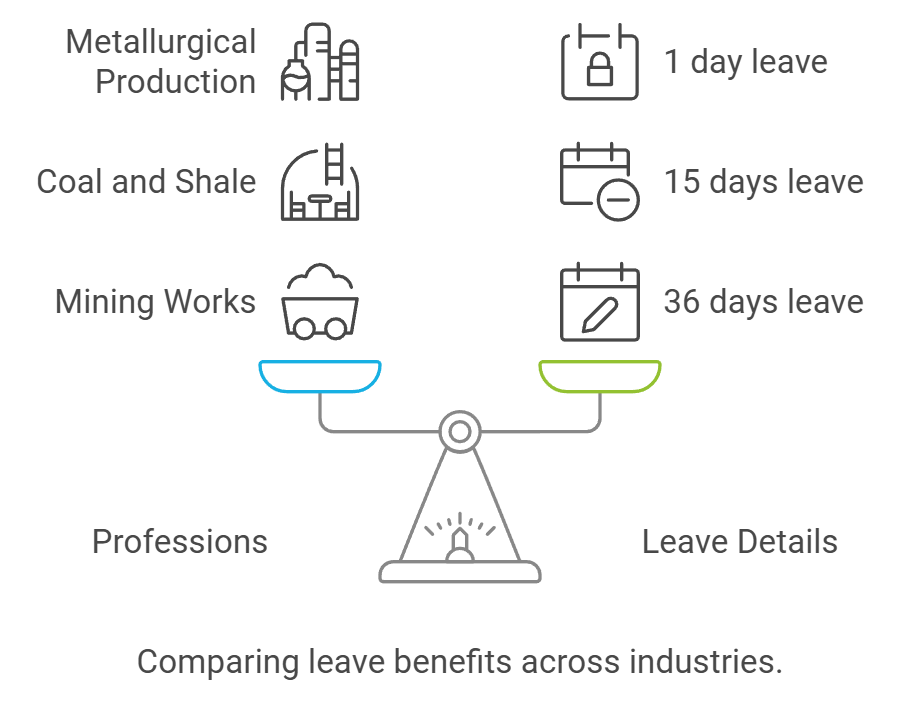
\includegraphics[width=0.5\textwidth]{media/gorn/image2}
	\caption*{Figure 1 - Comparing leave benefits across industries}
\end{figure}


\begin{multicols}{2}
{\bfseries Results and discussion.} The regulatory analysis of provisions for
guarantees to workers employed in heavy, hazardous, and dangerous
conditions in Kazakhstan revealed several key insights, focusing on the
so-called list-based approach. This approach defines guarantees based on
pre-established lists of professions, highlighting limitations in
adapting to contemporary labor conditions.

Under Article 1 of the Labor Code of the Republic of Kazakhstan, the
concept of «guarantees» refers to the means, methods, and conditions by
which the rights of workers in socio-labor relations are upheld.
Prescriptive guarantees for workers in hazardous or heavy labor
conditions are outlined in several provisions of the Labor Code (see
fig2)
\end{multicols}

\begin{figure}[H]
	\centering
	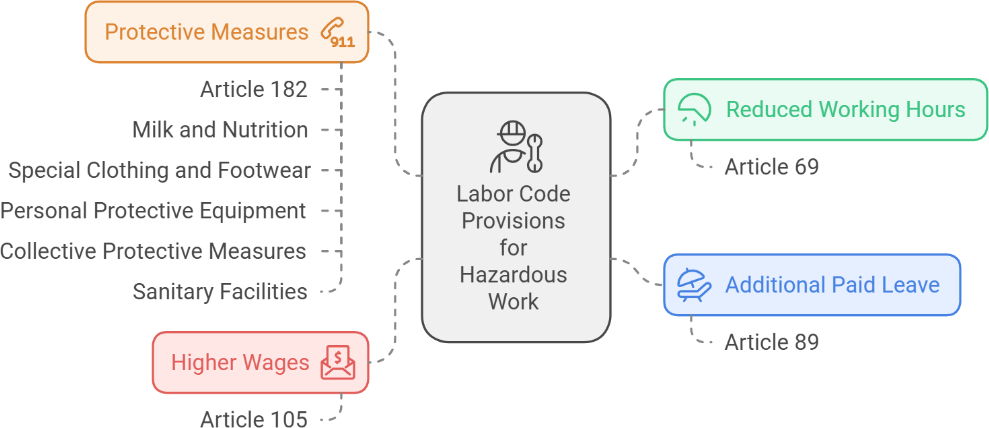
\includegraphics[width=0.8\textwidth]{media/gorn/image3}
	\caption*{Figure 2 - Social guarantees for employees working in hazardous labour conditions}
\end{figure}

However, it should be noted that these multiple legal instruments create
complexities in regulating safeguards for workers in hazardous
conditions, making it difficult to ensure consistent protection.
{\bfseries (}see fig 3)

\begin{figure}[H]
	\centering
	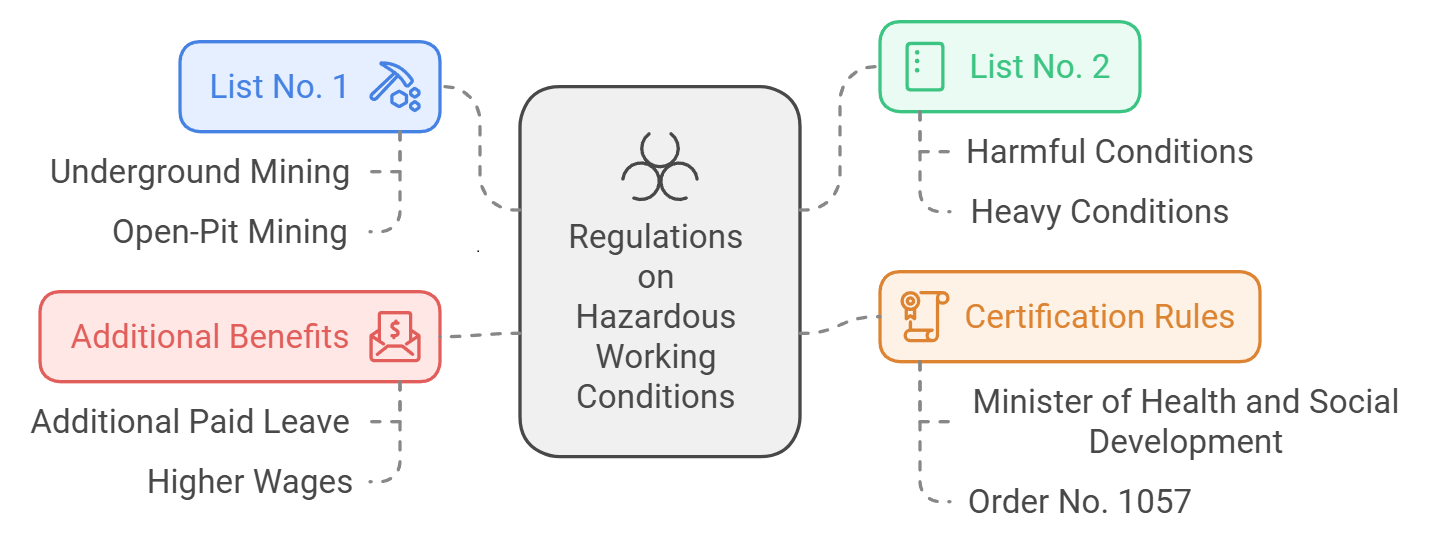
\includegraphics[width=0.8\textwidth]{media/gorn/image4}
	\caption*{Figure 3 - Legal instruments}
	\caption*{\emph{{\bfseries Social-Economic Challenges and Legal Barriers}}}
\end{figure}

\begin{multicols}{2}
The analysis identified socio-economic problems, legal barriers, and
restrictions in providing guarantees to workers employed in hazardous
conditions. Specifically, there are frequent complaints from workers
whose professions are not included in the prescribed lists. Comparative
analysis showed that some professions overlap, and discrepancies exist
within the lists, making it difficult to generate detailed analytical
data on expenses across professions.

The current practice revealed that a review of some types of social
guarantees is necessary. For instance, representatives from the oil and
gas sector suggested substituting milk with shubat or dietary
supplements, indicating a shift towards more relevant forms of
nutritional support.

Issues have also been identified in the assessment procedures of
production facilities. Often, submitted documents contain inaccurate
data, leading to erroneous managerial decisions and unnecessary economic
costs. This issue is tied to the poor quality of labor assessments and
the subjectivity of experts involved. In such cases, conscientious
employers fulfill their social guarantee obligations based on collective
agreements, which underscores the presence of legal barriers.

Experts, including representatives from the Republican Association of
Mining and Metallurgical Enterprises, have argued for abandoning the
list-based approach. With or without this approach, employers continue
to face significant financial burdens related to providing social
guarantees.

\emph{{\bfseries International Comparisons.}} An analysis of international
experiences showed that European Union countries have moved away from
compensation systems for hazardous and dangerous working conditions,
which remain in some post-Soviet states. EU countries avoid additional
payments for hazardous work, not due to a lack of understanding of their
motivational effect but based on ethical considerations - finding it
inappropriate to financially incentivize workers to accept known risks.

Most European countries have implemented legislative measures to
maintain workers'{} well-being, such as setting a
statutory workday length, guaranteed paid leave, minimum wage, and
employment security. In the USA, the Ethical Code of Industrial
Hygienists {[}24{]} excludes financial rewards for hazardous work,
advocating preventive measures instead. The US Occupational Safety and
Health Act emphasizes the joint responsibility of employees and
employers for ensuring safe working~conditions. (see fig 4)
\end{multicols}

\begin{figure}[H]
	\centering
	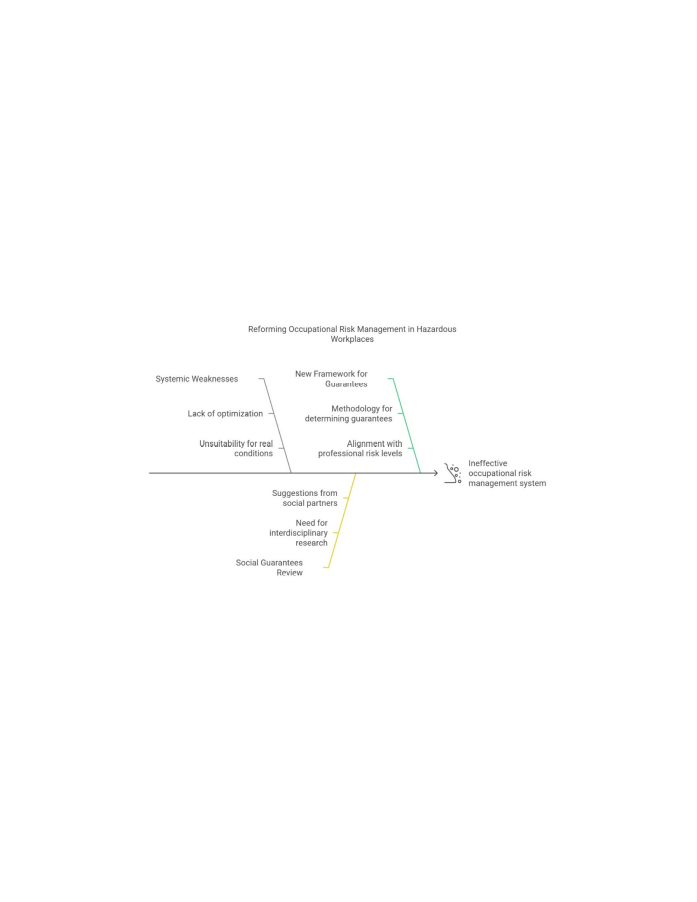
\includegraphics[width=0.8\textwidth]{media/gorn/image5}
	\caption*{Figure 4 - Transformation of the mechanism of social guarantees}
\end{figure}

\begin{multicols}{2}
The results of the study are presented below, refer to table 1.

{\bfseries Conclusions.} The current list-based system lacks optimization
and is unsuitable for adapting to the actual conditions faced by workers
in hazardous environments. There is a critical need for reform, moving
towards a model that factors in real-time assessments of occupational
risks. Revisiting the types of social guarantees offered is essential,
particularly nutritional provisions like milk, to adapt these measures
based on interdisciplinary research and the suggestions of social
partners, considering international experiences. The research resulted
in a proposal for a methodology to determine the volume of guarantees
for workers in hazardous conditions based on occupational risk
assessments. This risk-based approach will align social guarantees with
the level of professional risk present in each workplace, aiming to
provide equitable benefits tailored to the specific
needs~of~each~worker.

The analysis of the distribution of social guarantees across various
industries in Kazakhstan highlights significant disparities that reflect
the inefficiencies of the list-based approach. The data demonstrates a
need for more granular, risk-oriented policies that can better
accommodate the varying degrees of occupational hazards across sectors.
By transitioning to a risk-based model, Kazakhstan can enhance workplace
safety, ensure equitable treatment of workers, and foster a culture of
proactive risk management.
\end{multicols}

\begin{table}[H]
\caption*{Table 1. Key Insights from the Analysis of Occupational Safety Guarantees for Workers in Hazardous Conditions in Kazakhstan}
\centering
\begin{tblr}{
    colspec={|X[1]|X[2]|},
    hlines, vlines
}
\textbf{Category}                                             & \textbf{Findings}                                                                                                            \\
\textbf{List-based approach}                                  & Limited adaptability to modern labor conditions.                                                                             \\
\textbf{Socio-economic problems and legal barriers}           & Frequent complaints from workers not included in prescribed lists; overlapping professions; discrepancies.                   \\
\textbf{Assessment procedures issues}                         & Inaccurate data in assessment documents; poor quality of labor assessments and subjectivity of experts.                      \\
\textbf{International comparison (EU vs. USA)}                & EU countries avoid financial rewards for hazardous work, instead focusing on ethical considerations and preventive measures. \\
\textbf{Shift in nutritional support in hazardous conditions} & Shift from milk to shubat or dietary supplements in oil and gas sector to provide more relevant support.                     
\end{tblr}
\end{table}

\begin{multicols}{2}
This transformation requires regulatory reform, integration of advanced
risk assessment technologies, and the establishment of a culture that
values preventive measures over compensatory provisions. Moving forward,
stakeholders, including employers, government agencies, and labor
organizations, must collaborate to ensure that workers'{}
rights and safety are prioritized, ultimately contributing to fairer and
safer working~environments.

The research of current practices in advanced countries with a high
level of safe labour culture has shown the relevance of differentiating
the workplace by the degree of occupational risk and the scope of social
guarantees will depend on the degree of risk: high risk - full package
of guarantees.

The level of protection varies from a minimum level corresponding to a
low risk level to a maximum level at a very high risk level.

The new approach assumes that the type and scope of social guarantees
will be differentiated according to the degree of occupational risk.

Thus, the integral assessment of occupational risks (IAOR) is based on a
clear sequence of three indicators P1, P2 and P3. Where P1 is determined
automatically by the results of individual risk assessment of each
profession taking into account the specific weight of structural
subdivisions, P2 - Automatically analysed information by integrating AIS
«OTIB», HR.enbek.kz and stat.gov.kz, and P3 - determined by the results
of a check-list containing 15 questions, placed in the ODA module of AIS
«OTIB» by the employer, confirmed by the special organisation conducting
the integral assessment of occupational risks.

Thus, automation of analysis and control of the results of the IAOR will
allow solving a set of tasks: monitoring, analysis of indicators,
forecasting of the main trends, modernisation of reporting, formation of
a data bank, etc. This model provides for the automation of the
processes of identifying potential recipients of social guarantees,
minimising the risks associated with human participation in determining
the class of working conditions. Since all necessary data are integrated
from the systems of the state authorised labour body, employers.
According to the results of the IAOR, social guarantees will be assigned
only from the average class of labour conditions (3.2).

Effective management of occupational risks is impossible without
transformation of the state mechanism of social guarantees in respect of
persons employed in harmful working conditions. The essence of the new
ideology is that all elements of the safe labour system should be
interconnected and aimed at ensuring the implementation of the
constitutional right of every citizen of the Republic of Kazakhstan to
work in decent and safe working conditions.

It should be noted that the issue of integration of information systems
of mining and metallurgical enterprises was considered by Galiev S.J.,
Galiev D.A., Uteshev E.T., Tekenova A.T. {[}25

{]}, Edilbaeva L.I., Muzgina V.S., Mustapaev A.K. {[}26{]}.

\emph{{\bfseries Financing.} The article presents the results of the
research obtained in the course of implementation of the scientific and
technical programme «Transformation of the state mechanism of social
guarantees in respect of persons employed in harmful working conditions
in the modern context» (IRN BR22182673).}
\end{multicols}

\begin{center}
{\bfseries References}
\end{center}

\begin{references}
1. Bureau of national statistics agency for strategic planning and
reforms of the Republic of Kazakhstan //
\href{https://stat.gov.kz/ru}{https://stat.gov.kz/ru}. {[}in Russian{]}

2. Novikova \& Logachova, 2018 \href{https://www.researchgate.net/publication/328605049_Social_guarantees_for_persons_employed_in_industry_on_labour_conditions}{https://www.researchgate.net}

3. Smatlayev et al., 2023
\href{https://www.doi.org/10.32523/2616-6844-2023-144-3-42-50}{https://www.doi.org/10.32523/2616-6844-2023-144-3-42-50}

4. Abikenova et al., 2023
\href{http://vestnik.kuef.kz/web/uploads/file-vestnik/355030862d39f301e86c59a3e880429a.pdf}{http://vestnik.kuef.kz}

5. Рузанов et al., 2024
\href{https://sua.aesa.kz/main/article/view/222/192}{https://sua.aesa.kz}

6. Kalkayeva \& Moldakhmetova, 2022
\href{https://bulletin-law.kaznu.kz/index.php/journal/article/view/2663}{https://bulletin-law.kaznu.kz}

7. Chencheva, O., Sukach, S., Rieznik, D., Petrenko, I., Lashko, Y., \&
Hladiuk, O. (2024). Modern concept of occupational safety and health
management with a risk-based approach. Municipal Economy of Cities,
4(185), 221--227.
\href{https://doi.org/10.33042/2522-1809-2024-4-185-221-227}{https://doi.org}

8. Labour code of the Republic of Kazakhstan dated 23 November, 2015 №
414-V.

9. Resolution of the Government of the Republic of Kazakhstan dated
December 19, 1999, No. 1930 On the Approval of List No. 1 of Industries,
Jobs, Occupations, Positions, and Indicators for Underground and
Open-Pit Mining Work, Work with Particularly Hazardous and Particularly
Difficult Working Conditions, and List No. 2 of Industries, Jobs,
Occupations, Positions, and Indicators for Work with Hazardous and
Difficult Working Conditions {[}in Russian{]} //
\href{https://adilet.zan.kz/rus/docs/P990001930_/history}{https://adilet.zan.kz}

10. Order of the Minister of Healthcare and Social Development of the
Republic of Kazakhstan dated December 28, 2015, No. 1057 "On Approval of
the Rules for Mandatory Periodic Certification of \\Production Facilities
for Working Conditions"//
\href{https://adilet.zan.kz/rus/docs/V1500012743}{https://adilet.zan.kz}

11. Order of the Minister of Healthcare and Social Development of the
Republic of Kazakhstan dated December 28, 2015, No. 1053 "On the
Approval of the List of Industries, Workshops, Occupations, and
Positions, as well as the List of Heavy Work, Work with Harmful and (or)
Hazardous Working Conditions, Entitling Employees to Reduced Working
Hours, Additional Paid Annual Leave, and Increased Wages, and the Rules
for Granting These Benefits"//
\href{https://adilet.zan.kz/rus/docs/V1500012731}{https://adilet.zan.kz}.

12. Order of the Minister of Healthcare and Social Development of the
Republic of Kazakhstan dated December 28, 2015, No. 1054 "On the
Approval of the Rules for Providing Workers with Milk or Equivalent Food
Products and (or) Specialized Products for Dietary (Therapeutic and
Preventive) Nutrition, Special Clothing and Other Personal Protective
Equipment, Collective Protective Equipment, Sanitary and Domestic
Facilities, and Devices at the Employer' s Expense"//
\href{https://adilet.zan.kz/rus/docs/V1500012675}{https://adilet.zan.kz}

13. Resolution of the Government of the Republic of Kazakhstan dated
June 30, 2023, No. 520 "On the Approval of the Rules for Making
Mandatory Professional Pension Contributions" //
\href{https://adilet.zan.kz/rus/docs/P2300000520}{https://adilet.zan.kz}.

14. Wet van 23 november 1995, houdende bepalingen inzake de arbeids- en
rusttijden //\\\href{http://wetten.overheid.nl/jci1.3:c:BWBR0007671}{http://wetten.overheid.nl}.{[}in
Dutch{]}

15. Act of 18 March 1999, containing provisions to improve working
conditions (Working Conditions
Act)\href{https://www.businesslegalconsultancy.com/en/act-of-march-18-1999-containing-provisions-to-improve-working-conditions-act-on-working-conditions-1/}{https://www.businesslegalconsultancy.com}

16. Law on Financing of Social Insurance of 16 December 2004
\href{http://wetten.overheid.nl/jci1.3:c:BWBR0017745}{http://wetten.overheid.nl}

17. Law on Work and Income Depending on Capacity of 10 November 2005
\href{http://wetten.overheid.nl/jci1.3:c:BWBR0019057}{http://wetten.overheid.nl}

18. Law of the Republic of Lithuania dated September 14, 2016, No.
XII-2603 "On the Approval, \\Implementation, and Enforcement of the Labor
Code"
\href{https://e-seimas.lrs.lt/portal/legalAct/lt/TAD/bb10e743a97f11eb98ccba226c8a14d7?jfwid=kjtiqjlgg}{https://e-seimas.lrs.lt}.
{[}in Russian{]}

19. Law of the Republic of Lithuania dated July 18, 1994, No. I-549
"On State Social Insurance Pensions"
\href{https://e-seimas.lrs.lt/portal/legalAct/lt/TAD/TAIS.420452?jfwid=mmceok8cw}{https://e-seimas.lrs.lt}
{[}in Russian{]}

20. Resolution of the Government of the Republic of Lithuania dated
February 20, 1995, No. 267
"On the Approval of the Procedure for Calculating and Paying
Compensation for Special Working Conditions"
\href{https://e-seimas.lrs.lt/portal/legalAct/lt/TAD/TAIS.59421?jfwid=3d5v1wt4t}{https://e-seimas.lrs.lt}

21. Code du travail de la République française {[}in French{]}
\href{https://www.legifrance.gouv.fr/codes/texte_lc/LEGITEXT000006072050}{https://www.legifrance.gouv.fr}

22. European System of National and Regional Accounts //
\href{https://ec.europa.eu/eurostat/statistics-explained/index.php?title=European_system_of_national_and_regional_accounts_-_ESA_2010}{https://ec.europa.eu}

23. Fair Labor Standards Act//
\href{https://www.dol.gov/agencies/whd/flsa\#:~:text=The\%20Fair\%20Labor\%20Standards\%20Act\%20(FLSA)\%20establishes\%20minimum\%20wage\%2C,\%2C\%20State\%2C\%20and\%20local\%20governments}{https://www.dol.gov}.

24. Canons of Ethical Conduct and Interpretive Guidelines
\href{https://www.iloencyclopaedia.org/part-iii-48230/ethical-issues/item/1228-canons-of-ethical-conduct}{https://www.iloencyclopaedia.org}

25. Galiev S.Zh., Galiev D.A., Uteshov E.T., Tekenova A.T. O hode
cifrovizacii gorno-metallurgicheskogo kompleksa Kazahstana//Trudy-
Nauchno-tehnicheskogo obespechenija
gornogo proizvodstva.-2019.- T.89.- S. 251-258 {[}in Russian{]}

26. Edil' baeva L.I., Muzgiga V.S., Mustapaeva A.K.
Primenenie cifrovyh tehnologij dlja porvyshenija bezopasnosti gornyh
porod// Trudy- Nauchno-tehnicheskogo obespechenija gornogo
proizvodstva.- 2019.-T.89.-S.116-121 {[}in Russian{]}
\end{references}

\begin{authorinfo}
\emph{{\bfseries Information about the authors}}

Yensebayeva А. - Candidate of Legal Sciences, Head of Socio-Legal
Research Department, of the «Republican Scientific Research Institute
for Occupational Safety and Health of the Ministry of Labor and Social
Protection of the Republic of Kazakhstan»,Astana, Kazakhstan, е-mail:
\href{mailto:nel1212kz@gmail.com}{\nolinkurl{nel1212kz@gmail.com}};

Kurmanov А. - Candidate of Economic Sciences, General Director of the
«Republican Scientific Research Institute for \\Occupational Safety and
Health of the Ministry of Labor and Social Protection of the Republic of
Kazakhstan», Astana, Kazakhstan, е-mail: rniiot@rniiot.kz

Kazbekova D. - Institute of Industrial Ecological Sciences (IIES) of the
University of Occupational and Environmental Health, Japan, е-mail:
\href{mailto:kazbeken@med.uoeh-u.ac.jp}{\nolinkurl{kazbeken@med.uoeh-u.ac.jp}};
Aitimova Sh. - Head of the Economic Measurement and Statistics
Department of the «Republican Scientific Research Institute for
Occupational Safety and Health of the Ministry of Labor and Social
Protection of the Republic of Kazakhstan», Astana, Kazakhstan, е-mail:
\href{mailto:aitimova_80@mail.ru}{\nolinkurl{aitimova\_80@mail.ru}};

Yedilbayeva L. \emph{{\bfseries -}} Candidate of Medicine, Leading
Researcher, Branch «South» of the «Republican Scientific Research
Institute for Occupational Safety and Health of the Ministry of Labor
and Social Protection of the Republic of Kazakhstan»,Almaty, Kazakhstan,
е-mail:
\href{mailto:laura.ibragimovna@gmail.com}{\nolinkurl{laura.ibragimovna@gmail.com}}

\emph{{\bfseries Сведения об авторах}}

Енсебаева А. - кандидат юридических наук, заведующая отделом
социально-правовых исследований «Республиканского
научно-исследовательского института охраны труда и здоровья Министерства
труда и социальной защиты населения Республики Казахстан», Астана,
Казахстан, е-mail:
\href{mailto:nel1212kz@gmail.com}{\nolinkurl{nel1212kz@gmail.com}};

Курманов А. - кандидат экономических наук, генеральный директор
«Республиканского научно-исследовательского института охраны труда и
здоровья Министерства труда и социальной защиты населения Республики
Казахстан», Астана, Казахстан, е-mail: rniiot@rniiot.kz;

Казбекова Д. - Институт промышленных экологических наук (IIES)
Университета гигиены труда и окружающей среды, Япония, е-mail:
\href{mailto:kazbeken@med.uoeh-u.ac.jp}{\nolinkurl{kazbeken@med.uoeh-u.ac.jp}};

Айтимова Ш. - начальник отдела экономических измерений и статистики
«Республиканского научно-исследовательского института охраны труда и
здоровья Министерства труда и социальной защиты населения Республики
Казахстан», Астана, Казахстан,
е-mail:\href{mailto:aitimova_80@mail.ru}{\nolinkurl{aitimova\_80@mail.ru}};

Едильбаева Л. \emph{{\bfseries -}} кандидат медицинских наук, ведущий
научный сотрудник, филиал «Юг» «Республиканского
научно-исследовательского института охраны труда и здоровья Министерства
труда и социальной защиты населения Республики Казахстан»,Алматы,
Казахстан, е-mail:
\href{mailto:laura.ibragimovna@gmail.com}{\nolinkurl{laura.ibragimovna@gmail.com}}
\end{authorinfo}
